This section describes the various artifacts that will be generated during the project lifecycle. 

\subsection{Project Charter}
This will be stored in a GitHub repository where all team members will have access.
The charter will be updated upon unanimous agreement among the team.

\subsection{Product Backlog}
Any items that are necessary to complete the product. This will be updated when the team/product owner develops more knowledge throughout the implementation of the project. The Product Owner will be responsible for adding items to the Product Backlog. 

The Product Owner will be able to approve a feature another team member presents. The Product Owner must have the approval of at least one other member to add a new feature to the product backlog. The Product Owner can be outvoted by the other three team members if they unanimously agree.  

Removal of a feature requires the approval of two other team members (however, the current Scrum Master could alternatively just never assign it).

\subsection{Sprint Planning}
Sprint planning for the next Sprint will be in a group meeting within the last week of another sprint. Plans will be updated if there are any changes that require the team attention.

The Scrum Master will be in charge of approving which items are taken from the Product Backlog for each individual Sprint. He can only overrided if the other three team members unanimously agree.

\subsubsection{Sprint Goal}
The goal of each sprint is to successfully accomplish the main task of that sprint. This will be set and pushed by the Scrum Master, in accordance with the class's current goals.

\subsubsection{Sprint Backlog}
The Sprint backlog will hold the tasks for the current Sprint, which will be pulled from the Product Backlog. 

The Scrum Master will pull items from the Product Backlog for each sprint. The Scrum Master is unable to add new items without approval from the Product Owner.

\subsubsection{Task Breakdown}
Tasks will be distributed to team members when they are clearly defined. They will be posted on a digital Scrum Board where the team members will be allowed to assign themselves to the tasks. 

The Scrum Master is allowed to determine if a task requires more than one team member. The Scrum Master will also be allowed to remove a team member from a task if he is under performing.

If a task is currently unassigned, the Scrum Master is allowed to assign a team member accordingly.

\subsection{Sprint Burndown Charts}
WIP

\begin{figure}[h!]
    \centering
    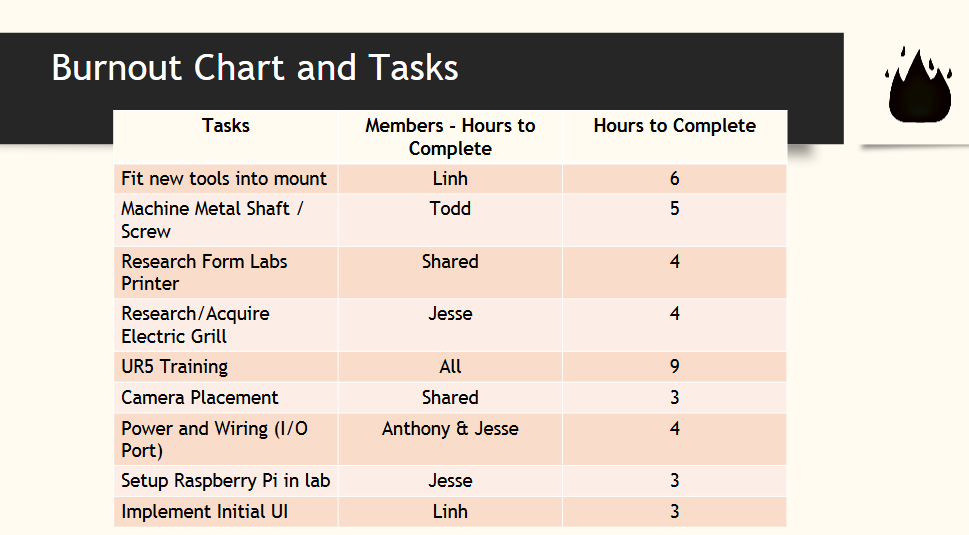
\includegraphics[width=0.5\textwidth]{images/Burndown_Chart}
    \caption{Example sprint burndown chart}
\end{figure}

\subsection{Sprint Retrospectives}
At the end of each sprint the team will be responsible for coming up with a retrospective for the Sprint to analyze what changes should be made for future sprints.

\subsection{Individual Status Reports}
N/A

\subsection{Engineering Notebooks}
Engineering Notebooks will be kept up to date and signed at the end of each week. If no additions are made to the Engineering notebooks, no signatures will be made.

\subsection{Closeout Materials}
The final documents that will be submitted will include this (Project Charter), the System Requirements Specification (SRS), the Architectural Design Specification (ADS), the Detailed Design Specification (DDS), and our Project Poster.

\subsubsection{System Prototype}
N/A

\subsubsection{Project Poster}
N/A (will be included with the final submission of this document)

\subsubsection{Web Page}
N/A

\subsubsection{Demo Video}
N/A

\subsubsection{Source Code}
N/A

\subsubsection{Source Code Documentation}
N/A

\subsubsection{Hardware Schematics}
N/A

\subsubsection{CAD files}
N/A

\subsubsection{Installation Scripts}
N/A

\subsubsection{User Manual}
N/A